\section{Contexto y decisiones}

La red atiende \emph{solicitudes}: encargos de recoger una cantidad de carga en un establecimiento de origen y entregarla en uno de destino el mismo día. Cada solicitud tiene una ventana para iniciar el retiro, una hora de apertura y un compromiso para terminar la entrega, y un tiempo máximo entre el fin del retiro y el fin de la entrega. La cantidad se mide en \emph{unidades de carga} (cajas o contenedores estandarizados), la misma unidad en que se expresa la capacidad de los vehículos. La semana completa de solicitudes se conoce de antemano.

Para atenderlas, la organización toma dos tipos de decisiones que se resuelven en conjunto, porque cada una condiciona a la otra:
\begin{itemize}\itemsep0pt
\item \textbf{Semanales:} qué vehículos contratar, en qué base queda cada uno toda la semana (desde allí sale y allí vuelve cada día) y qué puntos de transferencia (\emph{hubs}) habilitar.
\item \textbf{Diarias:} cómo se atiende cada solicitud, con qué vehículos y en qué orden recorre cada vehículo sus paradas.
\end{itemize}

Una solicitud se puede atender de cuatro formas. En el \emph{servicio directo}, un solo vehículo compatible la retira y la entrega. En la \emph{transferencia}, un vehículo la retira y la deja en un hub habilitado, y más tarde otro vehículo la recoge allí y la entrega; los vehículos no necesitan coincidir en el hub, basta con que el segundo llegue después de que el primero terminó la descarga. En la \emph{división}, la carga se reparte entre dos o tres vehículos distintos que viajan del origen al destino, lo que permite mover solicitudes que no caben en un solo vehículo. Por último, la solicitud se puede \emph{externalizar}, es decir, encargar a un transportista externo que cobra un monto fijo por solicitud. La externalización asegura la entrega, pero es la opción que la organización busca evitar porque es cara y deja la operación fuera de su control.

\section{Recursos y estructura de costos}

La flota tiene tres tipos de vehículo (Tabla~\ref{tab:flota}), que difieren en capacidad, en las clases de carga que pueden transportar y en costos. Los vehículos de un mismo tipo son idénticos. Además, la red dispone de bases, con un costo fijo semanal de \$130.000 a \$185.000 y capacidad para 5 a 8 vehículos, y de hubs, con un costo fijo de \$55.000 a \$85.000 por habilitarlos, un costo de manipulación de \$7.000 a \$10.000 por operación, un horario de 07:15 a 19:15 y una capacidad diaria de 24 a 32 operaciones.

\begin{table}[htbp]
\centering
\caption{Tipos de vehículo. La capacidad se mide en unidades de carga.}\label{tab:flota}
\small
\begin{tabularx}{\textwidth}{lccccY}
\toprule
Vehículo & Capacidad & Costo fijo semanal & Costo por km & Sobretiempo por min & Clases que transporta \\
\midrule
Van general & 30 & \$220.000 & \$550 & \$1.200 & Insumo general y equipo de retorno \\
Van fría & 24 & \$260.000 & \$650 & \$1.400 & Muestra clínica, fármaco refrigerado e insumo general \\
Furgón frío & 70 & \$380.000 & \$850 & \$1.700 & Las cuatro clases \\
\bottomrule
\end{tabularx}
\end{table}

El costo de una semana se compone de tres bloques. Los \emph{costos fijos} se pagan por cada vehículo contratado, cada base usada y cada hub habilitado, se use mucho o poco. Los \emph{costos variables de operación} dependen de las rutas: kilómetros recorridos, minutos de retorno a la base después de las 17:00 (sobretiempo), minutos de atraso en las entregas que lo admiten y manipulación en hubs. Finalmente, el \emph{costo de externalización} se paga por cada solicitud encargada a terceros. Las decisiones semanales fijan el primer bloque y las diarias los otros dos, pero los bloques se compensan entre sí: contratar un vehículo más cuesta entre \$220.000 y \$380.000 a la semana, y puede evitar varias externalizaciones de \$190.000 a \$250.000 cada una.

\section{Clases de carga}

Las solicitudes pertenecen a cuatro clases (Tabla~\ref{tab:clases}). La clase determina qué vehículos sirven, qué formas de atención se permiten, cuánto atraso se tolera y cuánto cuesta externalizar. Las muestras clínicas requieren custodia y bioseguridad y los fármacos, cadena de frío; por eso ambas viajan solo en vehículos refrigerados y no admiten atraso. Además, el fármaco refrigerado no puede viajar junto con insumo general.

\begin{table}[htbp]
\centering
\caption{Características y reglas de cada clase de carga.}\label{tab:clases}
\small
\begin{tabularx}{\textwidth}{lYYYY}
\toprule
 & Muestra clínica & Fármaco refrigerado & Insumo general & Equipo de retorno \\
\midrule
Cantidad (unidades) & 1--10 & 4--18 & 15--90 & 10--50 \\
Vehículos compatibles & Van fría, furgón & Van fría, furgón & Los tres & Van general, furgón \\
Transferencia & Sí & Sí & No & Sí \\
División & No & No & Sí, en 2 o 3 vehículos & No \\
Atraso permitido & No & No & Sí, \$800/min & Sí, \$1.200/min \\
Tiempo máximo de traslado & 165 min & 210 min & 300 min & 270 min \\
Costo de externalizar & \$230.000 & \$250.000 & \$190.000 & \$220.000 \\
No puede viajar con & -- & Insumo general & Fármaco refrigerado & -- \\
\bottomrule
\end{tabularx}
\end{table}

\section{Objetivos y entregable}\label{sec:objetivos}

El \textbf{objetivo general} es diseñar una metodología que coordine la planificación semanal de recursos con el ruteo diario de la red, al menor costo total y cumpliendo todas las restricciones operativas. De él se desprenden cinco objetivos específicos, que siguen los del enunciado del proyecto:
\begin{enumerate}\itemsep0pt
\item[O1.] Modelar y resolver el problema semanal integrado y compararlo con un caso base que represente la planificación por reglas (Capítulo~\ref{cap:trabajo}).
\item[O2.] Identificar los cuellos de botella: qué solicitudes son difíciles de atender, qué recursos limitan el desempeño y por qué (Sección~\ref{sec:resultados}).
\item[O3.] Evaluar la robustez de la solución ante cambios en la demanda, los tiempos de viaje, las ventanas, la flota, las bases y los costos (Capítulo~\ref{cap:sensibilidad}).
\item[O4.] Evaluar alternativas de expansión y reconfiguración: cerrar o abrir bases, dónde ubicar una base adicional y con qué vehículos, y agregar flota especializada (Sección~\ref{sec:infra}).
\item[O5.] Evaluar el aporte de la coordinación (transferencias y división) y cómo escala el método entre las instancias SMALL y BIG (Secciones~\ref{sec:small} y~\ref{sec:sensres}).
\end{enumerate}
El \textbf{entregable} es una herramienta computacional que, para una semana de solicitudes, entrega la flota contratada, la base de cada vehículo, los hubs habilitados, la forma de atención de cada solicitud y la ruta diaria de cada vehículo, junto con el costo desagregado y los indicadores de la Sección~\ref{sec:kpis}.

\section{Análisis de datos}\label{sec:datos}

Los datos tienen tres partes: un archivo transversal con la infraestructura, la flota y las reglas de cada clase; dos archivos de solicitudes, SMALL y BIG, con 10 instancias de 4 semanas independientes de 5 días hábiles cada una (80 semanas en total); y la red vial de la Región Metropolitana, un grafo de 142.000 nodos sobre el que se calculan tiempos y distancias. Las solicitudes usan siempre los mismos 103 establecimientos. La Tabla~\ref{tab:smallbig} compara ambos tamaños y la Figura~\ref{fig:mapa} muestra su geografía.

\begin{table}[htbp]
\centering
\caption{Comparación de las instancias SMALL y BIG (las 40 semanas de cada una).}\label{tab:smallbig}
\small
\begin{tabular}{lcc}
\toprule
 & SMALL & BIG \\
\midrule
Solicitudes por semana (mín.--máx.) & 258--364 & 455--731 \\
Solicitudes por día (mediana; máximo) & 60; 77 & 119; 154 \\
Flota: van general / van fría / furgón frío & 8 / 6 / 6 & 24 / 18 / 18 \\
Bases disponibles (cupos totales) & 5 (35) & 9 (62) \\
Hubs disponibles & 4 & 8 \\
Ventana de retiro, mediana & 90 min & 60 min \\
Retiros con ventana menor a 90 min & 21,7\,\% & 91,2\,\% \\
Ventana de entrega, mediana & 165 min & 120 min \\
Insumos generales sobre 70 unidades & 28,3\,\% & 37,7\,\% \\
Distancia media origen--destino por la red vial & 22,3 km & 27,0 km \\
\bottomrule
\end{tabular}
\end{table}

\begin{figure}[htbp]
\centering
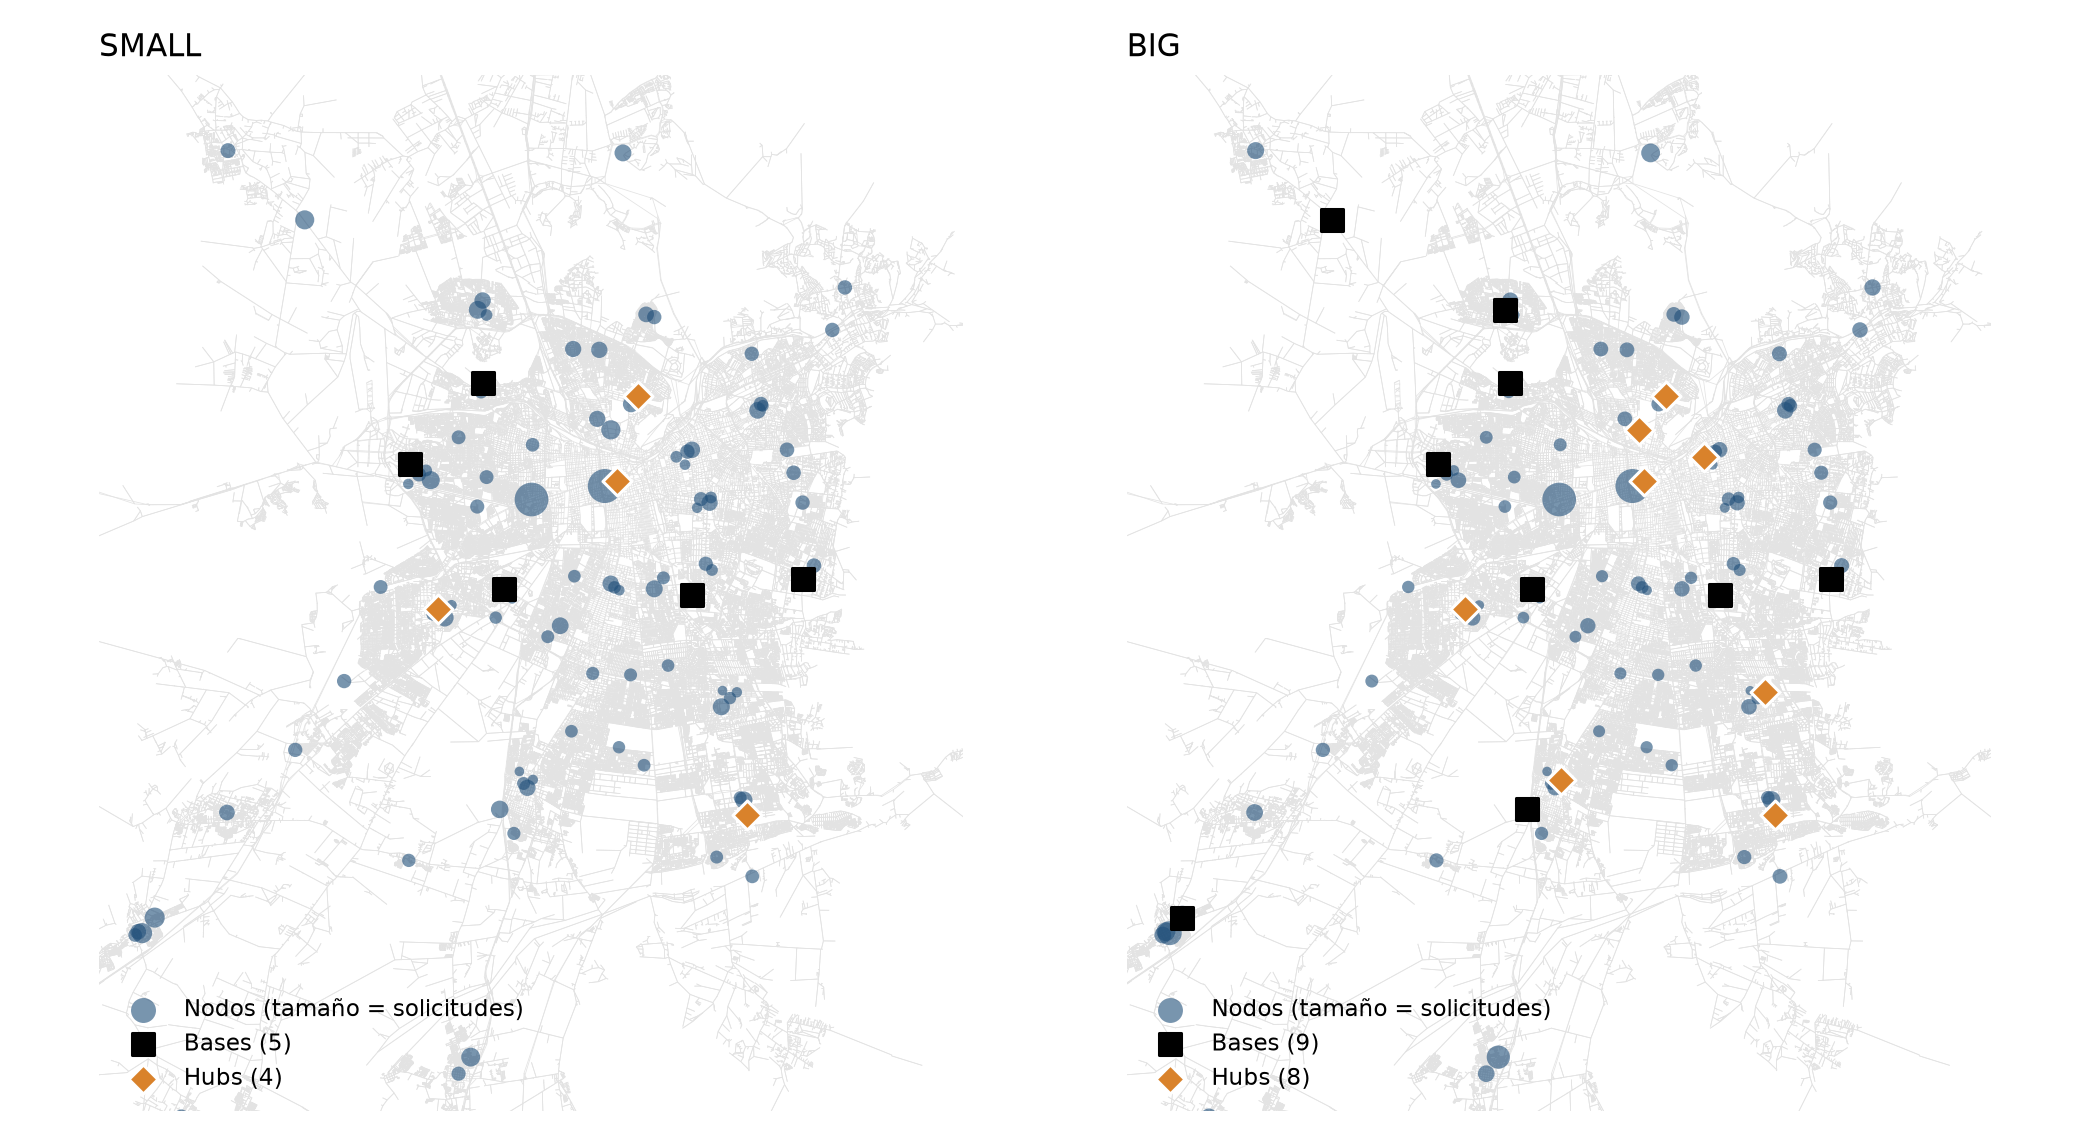
\includegraphics[width=0.92\textwidth]{figures/fig_mapa.png}
\caption{Establecimientos (tamaño según el número de solicitudes que los usan como origen o destino), bases y hubs disponibles en cada tamaño de instancia.}\label{fig:mapa}
\end{figure}

\parrafo{BIG no es solo más grande.} BIG tiene entre 1,8 y 2 veces las solicitudes de SMALL y exactamente el triple de flota, pero sus ventanas son mucho más estrechas: el 91\,\% de sus retiros tiene menos de 90 minutos para iniciarse, contra el 22\,\% en SMALL, y sus viajes son un 21\,\% más largos. La composición por clase, en cambio, es casi la misma: el insumo general es el 46,5\,\% de las solicitudes en SMALL y el 43,8\,\% en BIG, seguido por la muestra clínica (20,2 y 21,8\,\%), el equipo de retorno (19,2 y 20,1\,\%) y el fármaco refrigerado (14,1 y 14,3\,\%). La geografía es convergente: la demanda se reparte en la periferia, pero dos establecimientos del centro (Santiago Centro y Estación Central) concentran el 17,9\,\% de los destinos, lo que abre oportunidades de consolidar viajes hacia el centro.

\parrafo{La división es obligatoria, no opcional.} La Figura~\ref{fig:insumo} muestra que la distribución de cantidades del insumo general es bimodal. El 28,3\,\% de los insumos en SMALL y el 37,7\,\% en BIG supera las 70 unidades del furgón, el vehículo más grande, y por lo tanto solo se puede atender dividido o externalizado. Como el insumo es la única clase divisible, la división no es una mejora opcional sino una condición para no externalizar un tercio de los insumos.

\begin{figure}[htbp]
\centering
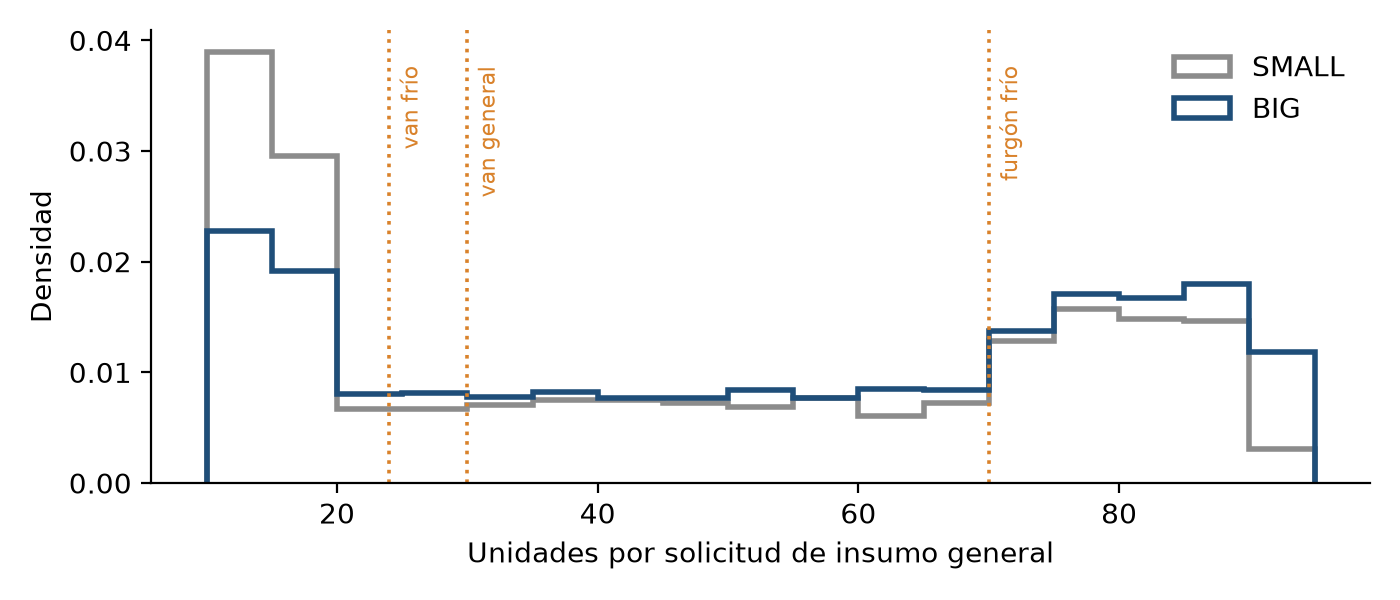
\includegraphics[width=0.72\textwidth]{figures/fig_insumo_capacidad.png}
\caption{Distribución de la cantidad de las solicitudes de insumo general y capacidad de cada tipo de vehículo.}\label{fig:insumo}
\end{figure}

\parrafo{Las ventanas concentran la demanda en pocas horas.} La Figura~\ref{fig:concurrencia} cuenta, cada 15 minutos, cuántas solicitudes están \emph{en curso}, es decir, ya abrieron su ventana de retiro y aún no vencen su entrega. Mientras están en curso, cada una necesita estar a bordo de algún vehículo o por ser recogida pronto. En lugar de un promedio, la figura muestra la mediana de los 200 días de cada tamaño y la banda entre los percentiles 10 y 90. En SMALL el máximo ocurre a las 14:45, con 34 solicitudes en curso en el día mediano y 48 en el peor, y supera la flota de 20 vehículos en los 200 días. En BIG el máximo se adelanta a las 10:00, cuando el día mediano iguala la flota de 60 vehículos y el peor llega a 97, y lo supera en el 70\,\% de los días. Como un vehículo puede llevar varias solicitudes a la vez, la flota alcanza, pero solo si las rutas consolidan bien en esas horas; por eso el costo depende tanto de la calidad del ruteo como del tamaño de la flota.

\begin{figure}[htbp]
\centering
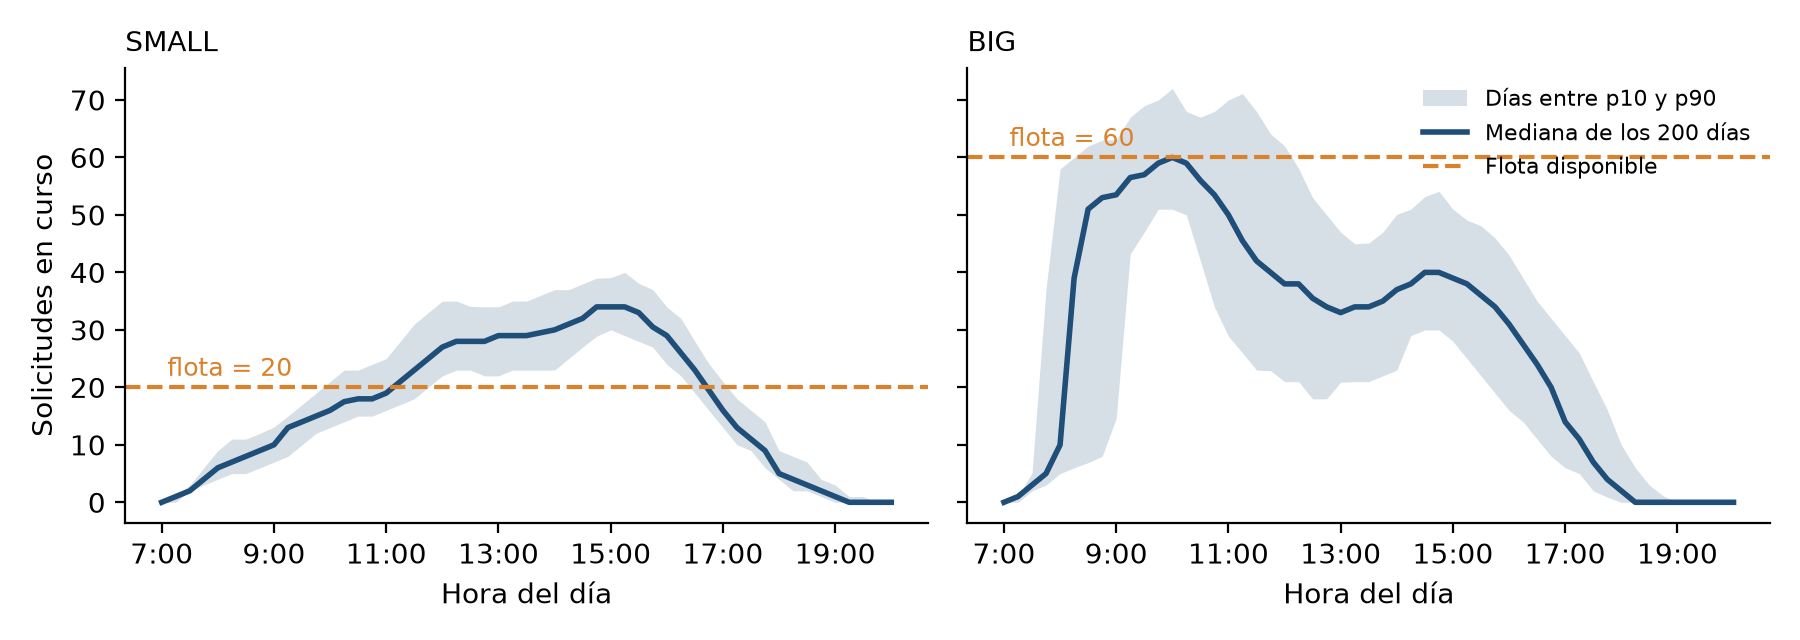
\includegraphics[width=0.92\textwidth]{figures/fig_concurrencia.png}
\caption{Solicitudes en curso a lo largo del día (entre la apertura de su retiro y el compromiso de su entrega), en los 200 días de cada tamaño de instancia.}\label{fig:concurrencia}
\end{figure}

\parrafo{El furgón es el recurso disputado.} El 34\,\% de las solicitudes en SMALL y el 36\,\% en BIG (muestras y fármacos) solo puede viajar en vehículos refrigerados, que son el 60\,\% de la flota. El furgón frío es el único vehículo compatible con las cuatro clases y el único que lleva insumos de más de 30 unidades sin dividir o equipos de más de 30 unidades, que son la mitad de los equipos. Es el más flexible, pero también el más caro de contratar y de operar: un furgón cuesta un 73\,\% más por semana que una van general y un 55\,\% más por kilómetro. Usarlo para cargas que caben en una van encarece la operación, mientras que reservarlo puede obligar a dividir o externalizar. Esa disyuntiva es una de las que la optimización tiene que resolver.

\parrafo{La incompatibilidad térmica limita la consolidación.} Se llama \emph{par expuesto} a una solicitud de fármaco y una de insumo del mismo día cuyos intervalos en curso se superponen, de modo que no pueden compartir vehículo en ese lapso. Hay en promedio 153 pares expuestos por día en SMALL y 503 en BIG. Como ambas clases pueden ir en vehículos refrigerados, esos pares obligan a separarlas justamente en los vehículos más disputados.

\section{Indicadores de desempeño}\label{sec:kpis}

La Tabla~\ref{tab:kpis} resume los indicadores con que se evalúan las soluciones. El costo total es el indicador principal y se reporta desglosado, porque un mismo total puede venir de estrategias muy distintas. Los demás indicadores explican de dónde viene el costo y verifican que una reducción no se logre a costa del servicio. Todos se calculan con el mismo código para el caso base y para la metodología propuesta.

\begin{table}[htbp]
\centering
\caption{Indicadores de desempeño y lo que permiten analizar.}\label{tab:kpis}
\small
\begin{tabularx}{\textwidth}{lYY}
\toprule
Área & Indicador y definición & Qué permite analizar \\
\midrule
Costo & Costo total semanal, desglosado en los bloques fijo, variable y de externalización; costo por solicitud. & Comparación económica global y origen del ahorro. \\
Servicio & Solicitudes externalizadas (número y \%); entregas atrasadas (\% de las atendidas). & Dependencia de terceros y cumplimiento de ventanas. \\
Recursos & Vehículos contratados por tipo; vehículo-días usados sobre vehículo-días pagados; fracción de la jornada usada; uso medio de la capacidad a bordo (carga media dividida por la capacidad, ponderada por kilómetro). & Tamaño y composición de la flota, capacidad ociosa. \\
Ruteo & Kilómetros por solicitud atendida; factor de recorrido (kilómetros recorridos divididos por la suma de las distancias origen--destino de las solicitudes atendidas); fracción de kilómetros en vacío; solicitudes por ruta. & Eficiencia de las rutas y nivel de consolidación. \\
\bottomrule
\end{tabularx}
\end{table}
